\documentclass[10pt]{article}%{scrartcl} % Beginn der LaTeX-Datei
\usepackage[utf8]{inputenc}  % für Unix-Systeme
\usepackage{amsmath,amssymb,mathtools}  % erleichtert Mathe 
\usepackage{tabularx}
\usepackage{enumerate}% schicke Nummerierung
\usepackage{geometry}
\geometry{a4paper,left=30mm,right=30mm, top=3cm, bottom=2cm} 
\usepackage{graphicx} % für Grafik-Einbindung
%\usepackage[dvips]{hyperref}
\usepackage{mdwlist}
\usepackage[labelfont=bf]{caption}
\usepackage{subcaption}
\usepackage{url}
\usepackage{grffile}

\usepackage[ngerman]{babel}
\addto\captionsngerman{\renewcommand{\figurename}{Abb.}}
%\usepackage[T1]{fontenc}
%\usepackage{lmodern}
 % Einstellungen, wenn man deutsch schreiben will, z.B. Trennregeln
  % ermöglicht die direkte Eingabe von Umlauten und ß
  % evt. obige Zeile ersetzen durch
  % \usepackage[utf8]{inputenc}
  % \usepackage[ansinew]{inputenc}  % für Windows
  % \usepackage[applemac]{inputenc} % für den Mac

%%%%%%%%%%%%%%%%%%%%%%%%%%%%%%%%%%%%%%%%%%%%%%%%%%%%%%%%%%%%%%%%%%
%
%  ntheorem
%
\usepackage[thmmarks,amsmath,hyperref,noconfig]{ntheorem} 
  % erlaubt es, Sätze, Definitionen etc. einfach durchzunummerieren.
\newtheorem{satz}{Satz}[section] % Nummerierung nach Abschnitten
\newtheorem{hilfssatz}[satz]{Hilfssatz}
\newtheorem{kor}[satz]{Korollar}

\theorembodyfont{\upshape}
\newtheorem{beispiel}[satz]{Beispiel}
\newtheorem{bemerkung}[satz]{Bemerkung}
\newtheorem{definition}[satz]{Definition}

\theoremstyle{nonumberplain}
\theoremheaderfont{\itshape}
\theorembodyfont{\normalfont}
\theoremseparator{.}
\theoremsymbol{\ensuremath{_\blacksquare}}
\newtheorem{beweis}{Beweis}
\qedsymbol{\ensuremath{_\blacksquare}}
%\theoremclass{LaTeX}
%
% Ende ntheorem
%
%%%%%%%%%%%%%%%%%%%%%%%%%%%%%%%%%%%%%%%%%%%%%%%%%%%%%%%%%%%%%%%%%%

%\pagestyle{empty}
%
% Ändern der bedruckten Fläche der Seite
% \addtolength{\textwidth}{3cm}  % Befehl mit zwei Argumenten
% \addtolength{\textheight}{3cm}
% \hoffset-2cm % verschiebt das Textfenster nach links
% \voffset-5mm % verschiebt das Textfenster nach oben
%
%\parindent=0pt %% keine Einzug zu Beginn von Abs\"atzen
%\parskip=2mm   %% erzeugt einen zusätzliche Zeilenabstand zwischen
                %% Absätzen. Nötig bei \parindent=0pt


\usepackage{pgf}
\usepackage{tikz}
\usetikzlibrary{arrows,automata,calc,patterns,positioning,shapes}


%%%%%%%%%%%%%%%%%%%%%%%%%%%%%%%%%%%%%%%%%%%%%%%%%%%%%%%%%%%%%%%%%%
%
%  ermöglicht, farbigen Text zu drucken.
%
\usepackage{color}
% Und nun werden die Farben definiert - daran können Sie nach Belieben selber rumspielen.
\definecolor{white}{rgb}{1,1,1}
\definecolor{darkred}{rgb}{0.3,0,0}
\definecolor{darkgreen}{rgb}{0,0.3,0}
\definecolor{darkblue}{rgb}{0,0,0.3}
\definecolor{pink}{rgb}{0.78,0.09,0.51}
\definecolor{purple}{rgb}{0.28,0.24,0.55}
\definecolor{orange}{rgb}{1,0.6,0.0}
\definecolor{grey}{rgb}{0.4,0.4,0.4}
\definecolor{aquamarine}{rgb}{0.4,0.8,0.65}


\DeclareMathOperator{\GL}{GL} % einige Macro, siehe am Ende Abschn. 2
\newcommand{\N}{\mathbb{N}}
\newcommand{\Z}{\mathbb{Z}}
\newcommand{\Q}{\mathbb{Q}}
\newcommand{\R}{\mathbb{R}}
\newcommand{\PP}{\mathbb{P}}
\newcommand{\PPX}{\mathbb{P}^X}
\newcommand{\C}{\mathbb{C}}
\newcommand{\cP}{{\mathcal P}} 

\setlength{\parindent}{0cm}
\setlength{\parskip}{.2cm}
\setlength{\fboxsep}{0pt}
%\setlength{\fboxrule}{.2mm}

%\usepackage{showframe}

\begin{document}

\author{Gruppe 04 -- Alex Oks, Markus Görlich, Simon Stieber}
\title{Selbstorganisierende, adaptive Systeme - Blatt 01}
%\date{} %hier können Sie ein Datum eingeben, auch leer, sonst wird es
         %automatisch erzeugt

\maketitle % erzeugt den Kopf
%%\let\clearpage\relax
\section{Aufgabe 1a}
Siehe Code in Ordner Aufgabe-01.
\section{Aufgabe 2a}
Weitere Beispiele für selbstorganisierende Systeme sind:
\subsection{Termitennester --- a}
Wie von Camazine beschrieben\footnote{Camazine, Bird flocks, zebra stripes, honeybee swarms:
	Self-organization in biological systems, \url{http://order.ph.utexas.edu/Camazine.pdf}, Abgerufen am 24.10.16}
erzeugen Termitenvölker höchst komplexe Bauten für ihren Stamm.
Es gibt Kamine, Säulen, Windräder, eine Kammer für die Königin, Pilzgärten, Belüftungen und Keller.
In diesem komplexen Gebilde können Temperatur und Feuchtigkeit kontrolliert werden, es bietet Schutz und verschiedene Materialien können aufbewahrt/konserviert werden.
Außerdem wird für einen ständigen Luftaustausch gesorgt.

Diese erstaunlichen Fähigkeiten ihres Gebäudes werden von sehr primitiven Wesen erzeugt --- Termiten.
Wie geht das?
Soziale Insekten haben einfache Verhaltensregeln entwickelt um diese Architekturen zu erzeugen.

%Beispiel Activation-Inhibition Mechanismus.
%TODO wie genau muss das sein?
\subsection{Termitennester --- b}
\paragraph{Agenten}
Viele Termiten, die nach und nach ein sehr komplexes Gebäude errichten.
Sie werden nicht zentral gesteuert sondern arbeiten anhand lokaler Gegebenheiten:
Was machen die anderen Termiten, Kommunikation mit anderen Termiten.
\paragraph{Einfluss der Umwelt auf das System}
Schutz der Termiten und der Königin vor der Umwelt (Wetter/feindliche Tiere) durch das Gebäude.
\paragraph{Interaktionen zwischen Agenten}
Lokale Kommunikation zwischen den Termiten
\paragraph{Interaktionen zwischen Agenten und Umwelt}
Bauen eines Gebäudes aus dem was da ist, dem Boden.
\subsection{Vogelschwärme --- a}
TBD\footnote{Tanner et al., Stable Flocking of Mobile Agents, Part I: Fixed
	Topology, \url{http://ieeexplore.ieee.org/document/1272910/}, Abgerufen am 24.10.16}
\subsection{Vogelschwärme --- b}
TBD
\section{Aufgabe 3}

\subsection{Verhalten ohne disease und grow}
Ohne disease und grow steigt die Anzahl an Turtles zu Begin der Simulation und die Anzahl der Grasfelder sinkt. Nach etwa 20 Ticks beginnen die Werte sich auf 350 turtles und 120 grass einzupendeln. (Siehe Abb. 1) 


\subsection{Verhalten mit disease 30}
Mit einem disease-Wert von 30 und wiederholtem drücken des disease-Buttons fällt die Anzahl der Turtles auf ca 120 herab und die Anzahl der Grasfelder steigt auf ungefähr 350 an. Auch wenn der disease-Button weiterhin gedrückt wird ändern sich die Werte kaum. Nachdem der disease-Button nicht mehr gedrückt wird, pendelt sich die Anzahl der Turtles und Grasfelder langsam wieder auf die Werte ein, die im Versuch ohne disease und grow erreicht wurden. (Siehe Abb. 1)  


\subsection{Verhalten mit disease 40}
Mit einem disease-Wert von 40 und wiederholtem drücken des disease-Buttons fällt die Anzahl der Turtles auf ca 25 herab und die Anzahl der Grasfelder steigt auf ungefähr 650 an. Man sieht, dass die Turtles in diesem Szenario fast komplett aussterben und die Grasfelder fast an allen Stellen wieder nachgewachsen sind.
Trotz der gewaltigen Dezimierung der Turtles, wächst ihre Population nach dem Krankheitsbefall wieder auf die Werte des ersten Szenarios an. (Siehe Abb. 1) 


\subsection{Verhalten mit grow}
Bei wiederholtem Drücken des grow-Buttons zeigt sich, dass die Anzahl der Turtles enorm steigt. Die Anzahl der Grasfelder sinkt nach einem kurzen Anstieg aber sofort wieder. Nach der Regenphase sinkt die Population der Turtles wieder auf ihren Ausgangswert. (Siehe Abb. 1) 

\subsection{Verhalten mit disease und grow}
Wenn Wachstum und Krankheit zeitlich zusammenliegen, pendeln sich die Werte für die Anzahl der Turtles und die Anzahl der Grasfelder sehr schnell wieder auf ihre Ausgangswerte ein. Grow und disease gleichen sich gegenseitig aus. (Siehe Abb. 1) 


\begin{figure}
	\centering
  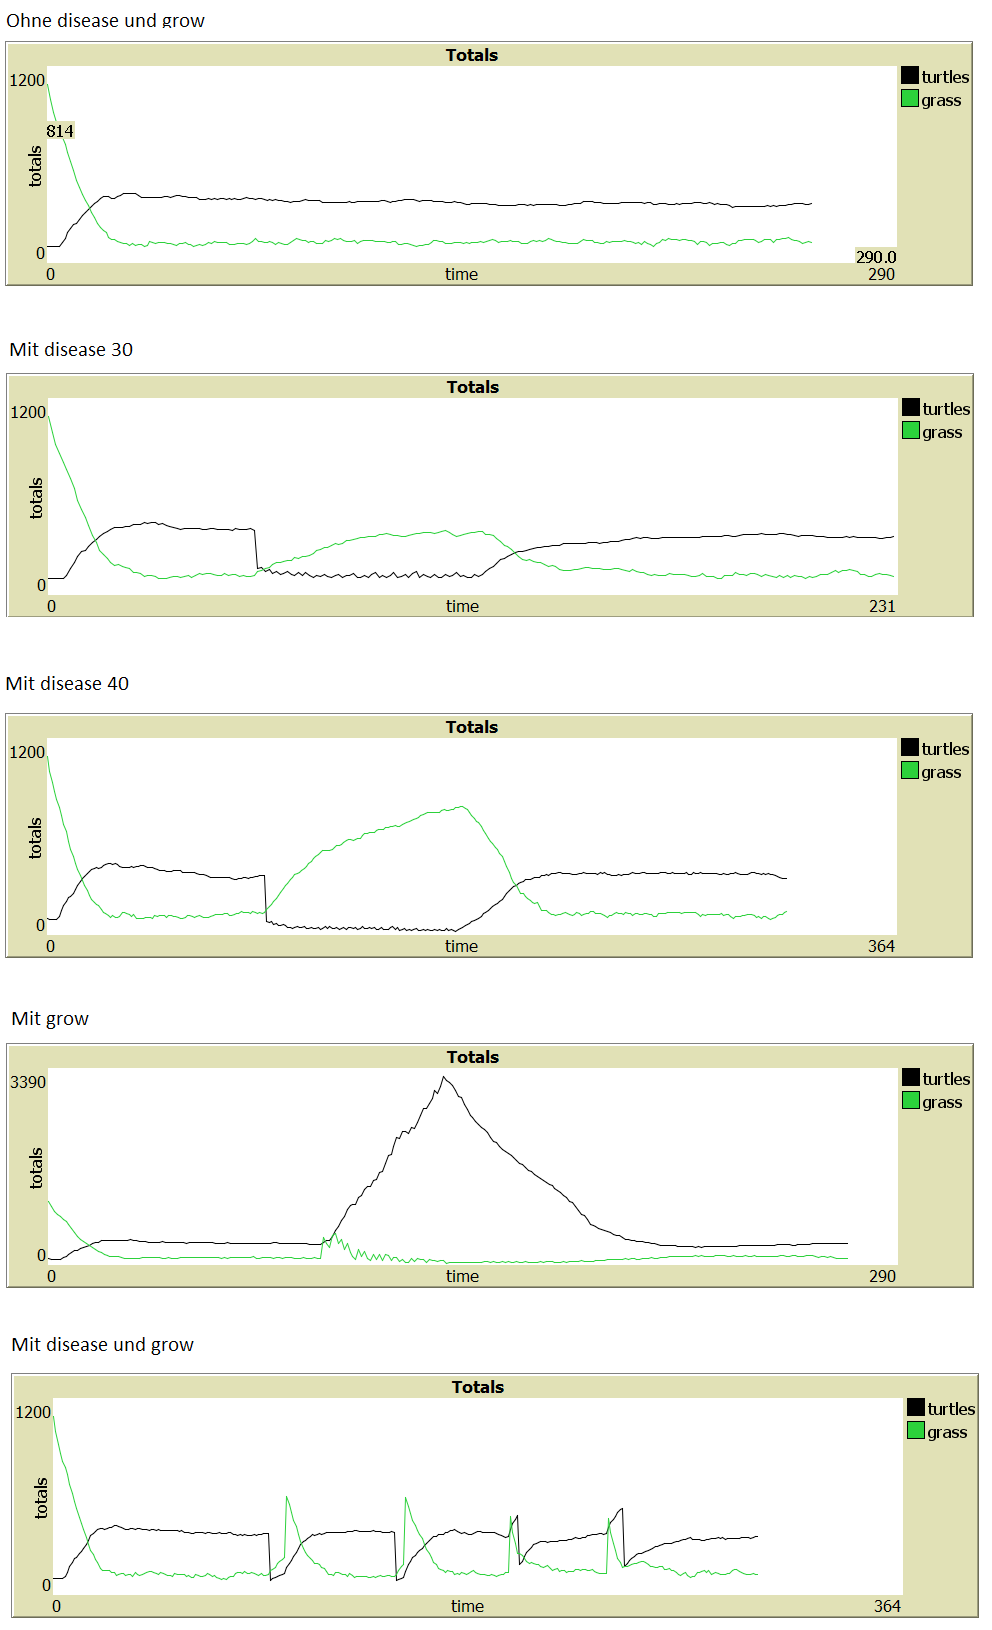
\includegraphics [scale = 0.56]{Blatt 1 - 3 Bild.png}
\caption{Versuche Aufgabe 3}
\label{Abb1}
\end{figure}
\end{document}